\documentclass{article}
\usepackage{caption}
\usepackage{subcaption}
\usepackage{hyperref}
\usepackage{graphicx}
\usepackage{amsmath}
\usepackage[utf8]{inputenc}
\usepackage[margin=1in]{geometry}

\title{Real-time Diagnostic Tools for the Scanning Electron Microscope}
\author{Liuchuyao Xu\\Robinson College}
\begin{document}
\maketitle
\tableofcontents
\newpage

\section{Introduction}
\subsection{Project Objectives}
The scanning electron microscope (SEM) is a type of microscope that produces images using signals generated from the interaction between electrons and the surface under observation. Higher resolution can be achieved compared to the traditional optical microscope, since electrons have much lower wavelength than light. An SEM can have resolution lower than one nanometre, whereas that of an optical microscope is often limited to a few hundred nanometres \cite{SEM wiki}. This has benefited a variety of fields. For example, scientists have been using the SEM to analyse the doping density in semiconductor \cite{SEM for semiconductor}. The goal of the project is to develop software tools in Python to support diagnosis of SEM images for the purpose of assisting the operator or automating procedures.

\subsection{Theory of the SEM}
Figure \ref{SEM basic construction} shows the basic construction of an SEM. The electron gun generates an electron beam, which is transformed into an electron probe after passing through the condenser lens and objective lens. It is scanned across the specimen under the effect of the scanning coil. As a result of the interaction between the incident electrons and the specimen, some electrons are emitted from the specimen. These are called secondary electrons and are collected by the detector, which generates signals whose magnitude depend on the strength of the secondary electrons. The display unit produces one frame after each complete scan of the specimen.

\begin{figure}
    \centering
    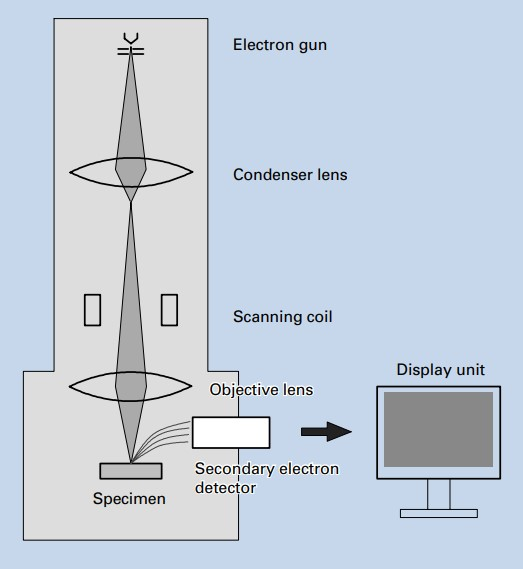
\includegraphics[width=0.9\textwidth]{Images/SEM basic construction.jpg}
    \caption{Basic construction of an SEM \cite{SEM A to Z}}
    \label{SEM basic construction}
\end{figure}

\subsection{How Fast Computing Can Aid SEM Operators}
The quality of an SEM image is affected by aberrations. While some exist because of the fundamental properties of the microscope and are difficult to get rid of, some can be completely eliminated by adjusting relevant settings. Two important ones are focus and stigmation, which directly affect the resolution and astigmatism of the image, respectively. Figure \ref{Sample SEM images} illustrates the effect of wrong focus and stigmation settings.

Focus determines the focal point of the electron probe. When the focal point is far from the surface of the specimen, the incident electrons interact with the specimen in a larger area. As a result, spots near each other produce signals of closer magnitude. This makes the image appear blurry, as shown in Figure \ref{A out of focus}.

Stigmation controls stigmators in the SEM, which are used to compensate for astigmatism. Astigmatism arises due to imperfections in components of the SEM, and describes uneven focus in the electron probe, as shown in Figure \ref{SEM uneven focus}. When the electron probe is out of focus, astigmatism makes the incident electrons interact with the specimen in an elliptical area, and thus makes the image appear stretched. When the electron probe is in focus, astigmatism makes the image appear blurry. Figure \ref{Sample astigmatic SEM images} gives some examples of distorted images.

\begin{figure}
    \centering
    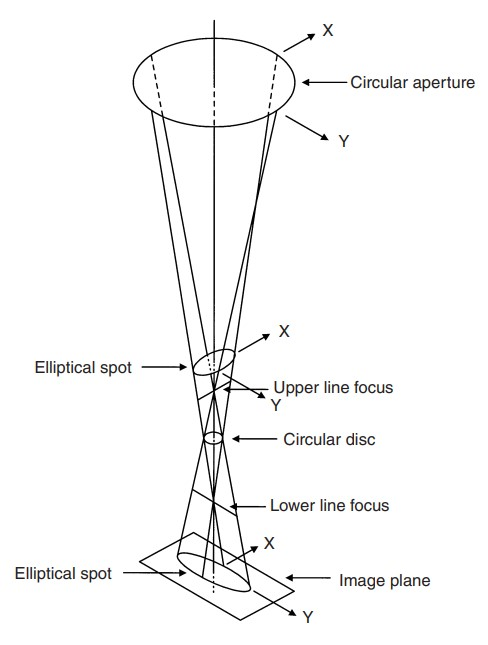
\includegraphics[width=0.3\textwidth]{Images/SEM uneven focus.jpg}
    \caption{Uneven focus of the SEM}
    \label{SEM uneven focus}
\end{figure}

\begin{figure}
    \centering
    \begin{subfigure}{\textwidth}
        \centering
        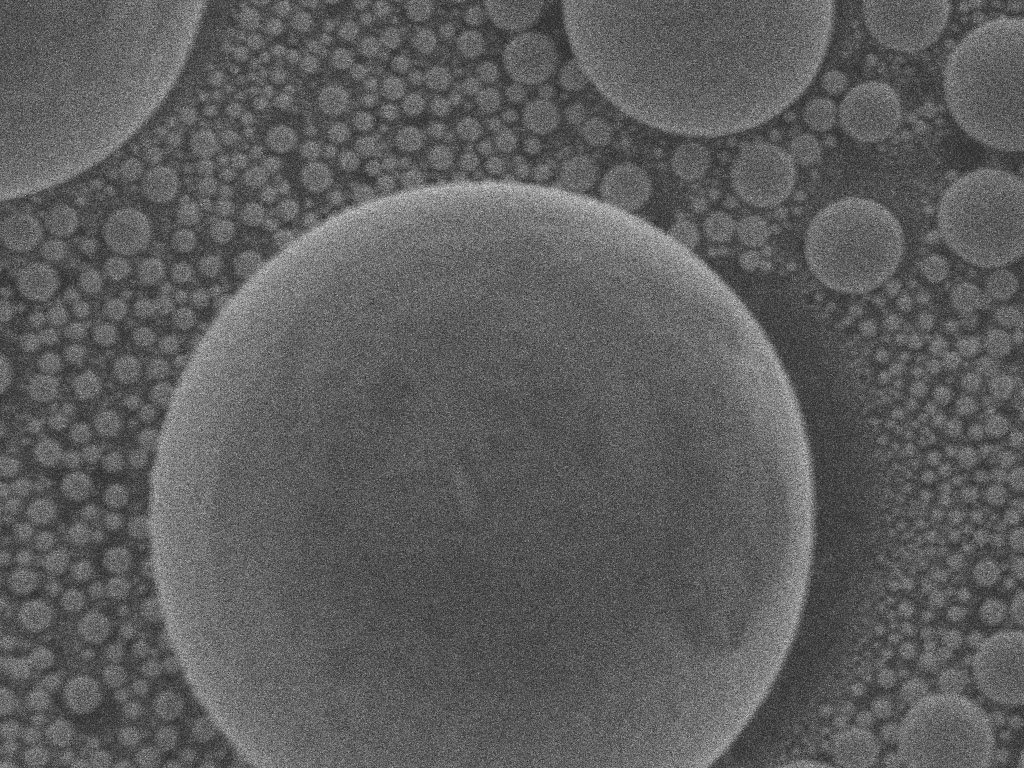
\includegraphics[width=0.3\textwidth]{Images/A in focus.jpg}
        \caption{In focus}
        \label{A in focus}
    \end{subfigure}
    \begin{subfigure}{\textwidth}
        \centering
        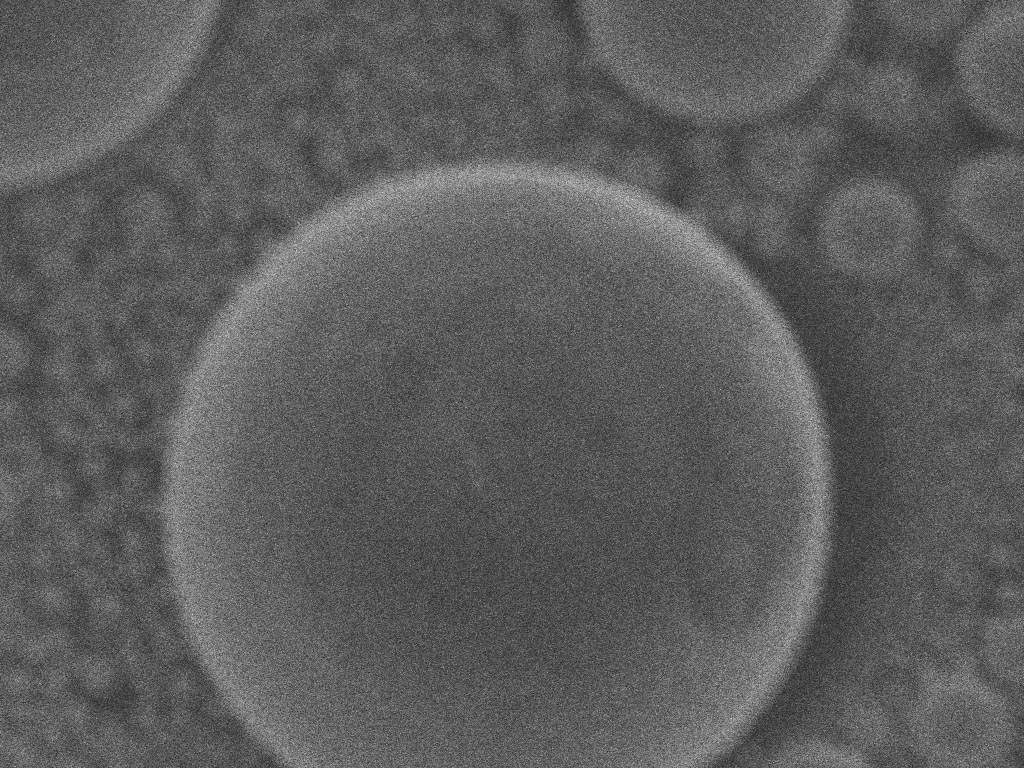
\includegraphics[width=0.3\textwidth]{Images/A out of focus.jpg}
        \caption{Out of focus}
        \label{A out of focus}
    \end{subfigure}
    \begin{subfigure}{\textwidth}
        \centering
        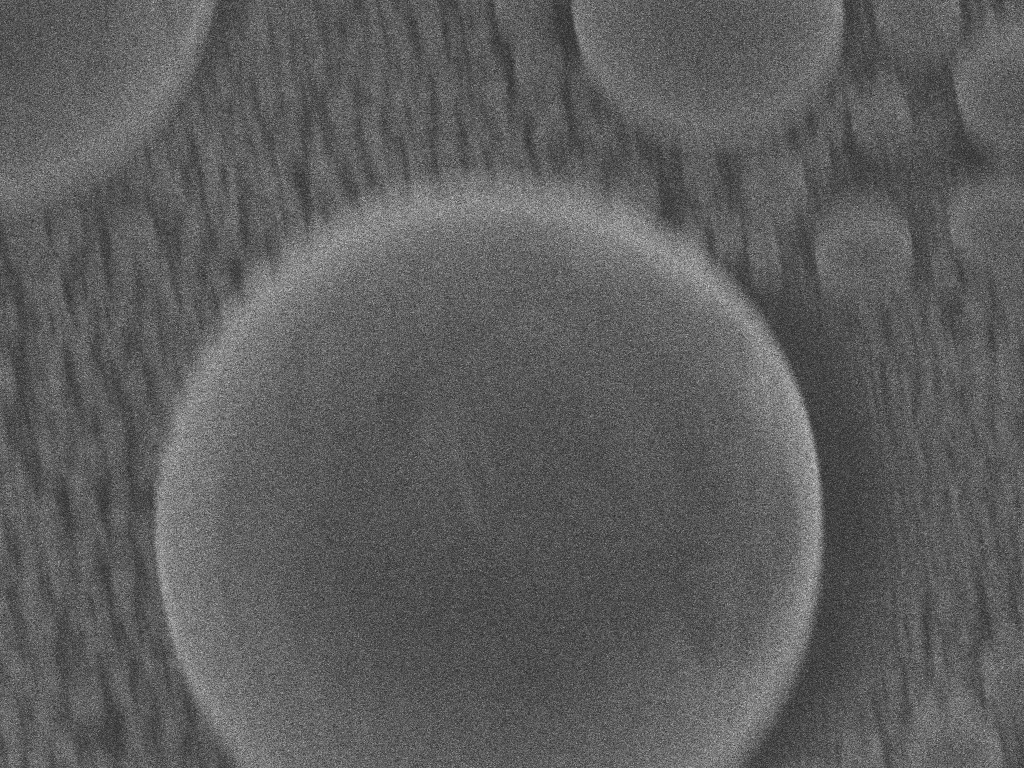
\includegraphics[width=0.3\textwidth]{Images/A astigmatism.jpg}
        \caption{In focus with astigmatism}
        \label{A astigmatism}
    \end{subfigure}
    \caption{Sample SEM images}
    \label{Sample SEM images}
\end{figure}

\begin{figure}
    \centering
    \begin{subfigure}{\textwidth}
        \centering
        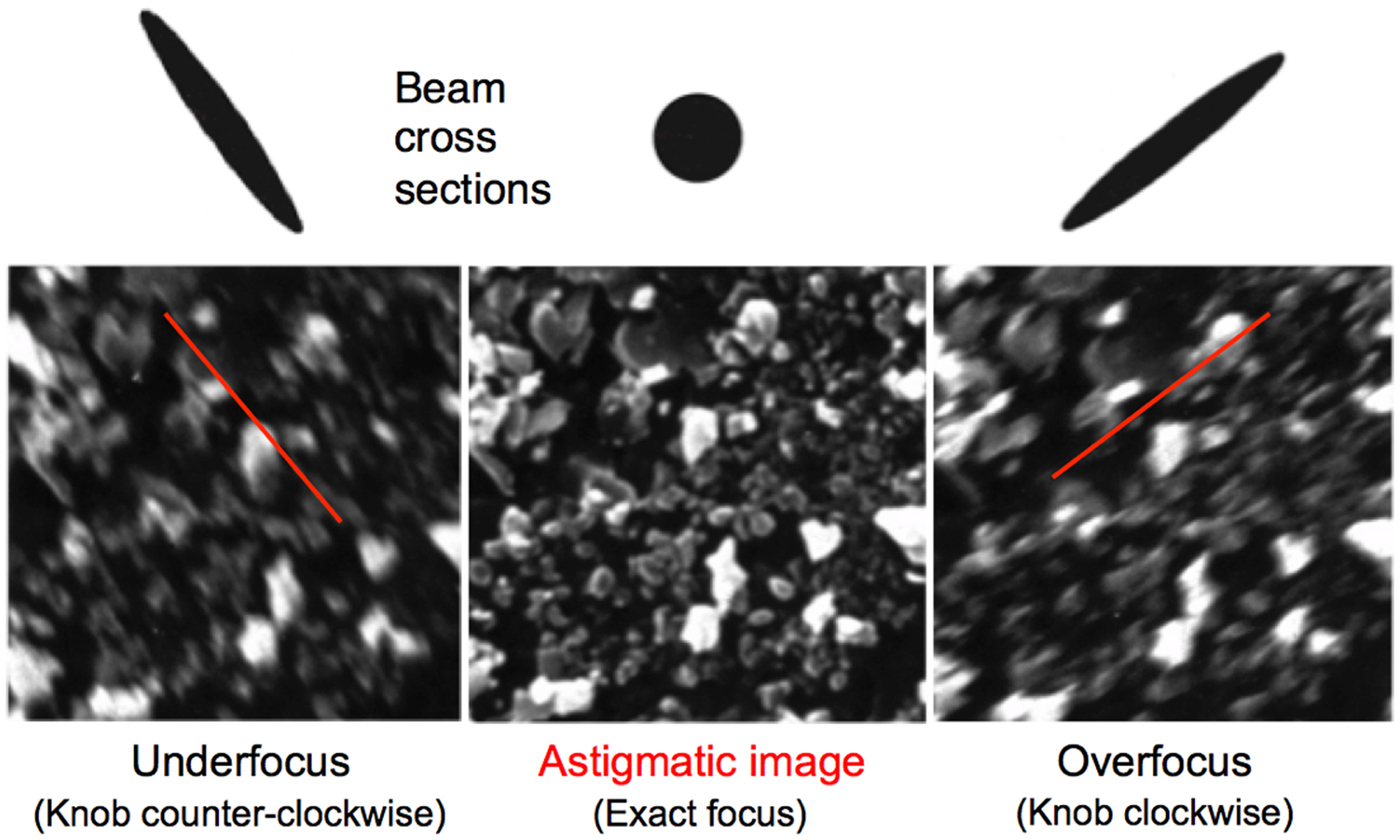
\includegraphics[width=0.3\textwidth]{Images/B astigmatic a.jpeg}
        \caption{Astigmatic images}
        \label{B astigmatic a}
    \end{subfigure}
    \begin{subfigure}{\textwidth}
        \centering
        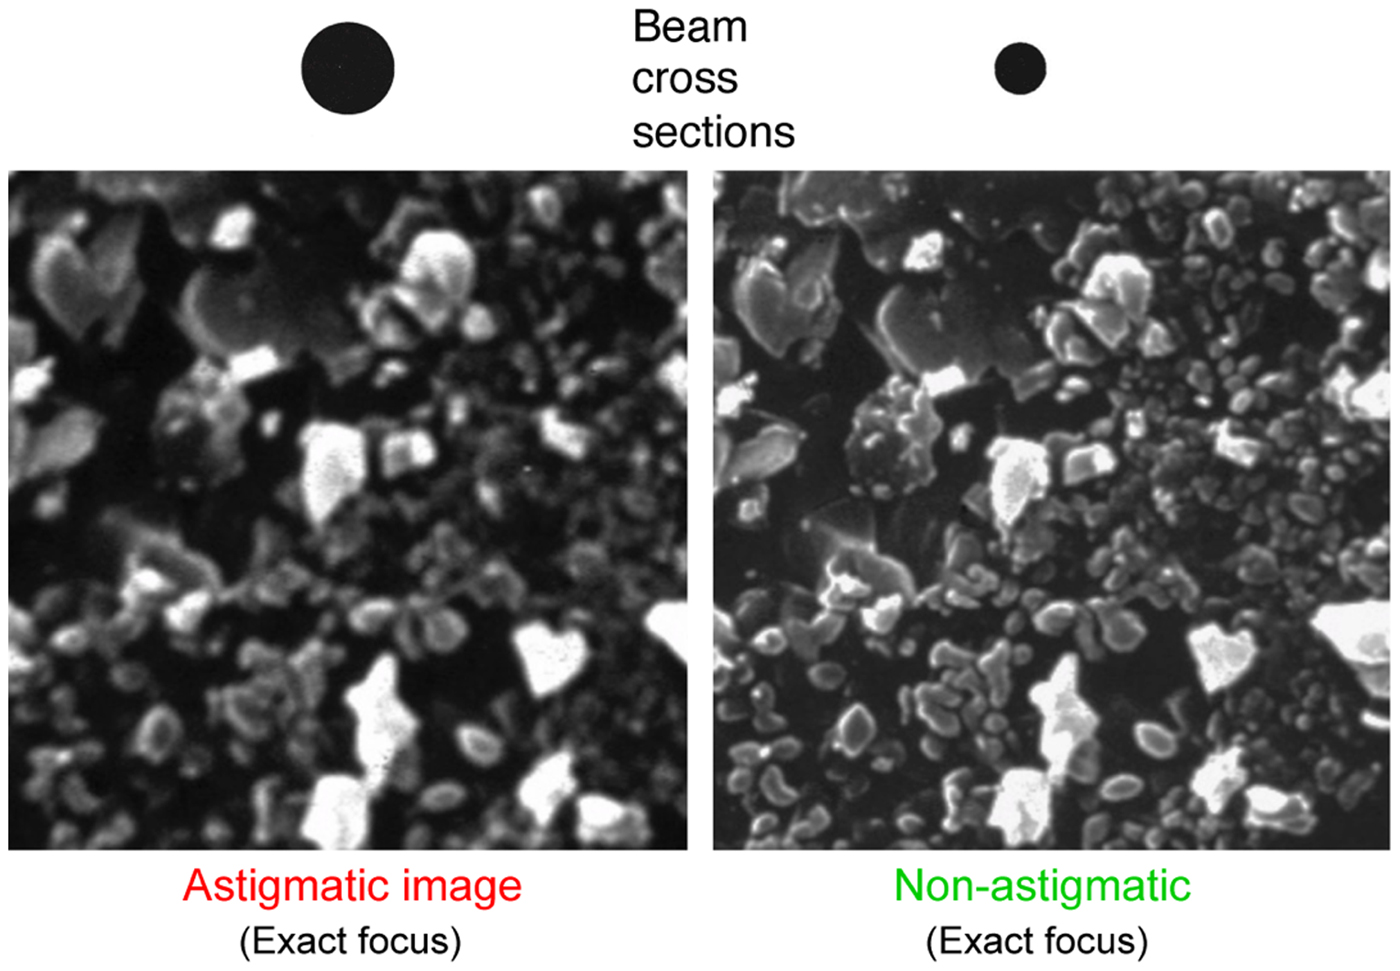
\includegraphics[width=0.3\textwidth]{Images/B astigmatic b.jpeg}
        \caption{Astigmatic and non-astigmatic image}
        \label{B astigmatic b}
    \end{subfigure}
    \caption{Sample astigmatic SEM images \cite{SEM astigmatism correction}}
    \label{Sample astigmatic SEM images}
\end{figure}

Although experienced SEM operators can often find the right settings for focus and stigmation in a short time, it may not be as straightforward for new users. Sometimes, the surface being observed may have a complex structure and makes adjusting even harder. The complexity arises because any judgement of an image is based on what the operators see through their eyes, which is rather subjective. Intensive training and practical experience are often required for an operator to become efficient in using the SEM.

Fast computing can aid the operators in a few ways. Firstly, a numerical evaluation of the quality of the image may be provided, which eliminates the subjectivity in using human eyes. Numbers are also easier to note down if any record is required. Two operators may have different views on the same image, but the numbers will not be different. Therefore, cooperation and communication between operators can be enhanced. The use of numbers also enable automatic procedures for adjusting settings of the SEM, which save time and may produce better results than doing it manually.

The project focuses on developing tools that use Fast Fourier Transform (FFT) to help operators evaluate the focusing and astigmatism of SEM images, and also looks into an algorithm for the automatic correction of them.

\section{The Algorithms}
\subsection{Histogram Equalisation}
There are many types of histograms in image processing. The grey level (brightness level) pixel intensity histogram, which plots the number of pixels of each grey value in the image, is the most relevant one for SEM images. This is because an SEM translates the energy of the secondary electrons directly into a grey level, colours do not exist in SEM images.

The algorithm for obtaining the histogram of an SEM image is given by
\begin{equation}
    n_l = \frac{1}{P} \sum_{p} I(l_p=l)
\end{equation}
where $n_l$ is the normalised number of pixels of grey level $l$, $P$ is the total number of pixels in the image and $l_p$ is the grey level of the $p_{th}$ pixel. 

Figure \ref{C original} shows an 8-bit grey-scale image, i.e. its depth of digitisation is 8-bit and it has 256 grey levels. Figure \ref{C original histogram} shows the histogram of the image and its integral. As can be seen in the histogram, most pixels are concentrated in the middle of the grey scale. This is reflected by the fact that the image is missing its highlights and shadows.

Histogram equalisation is a method for adjusting the distribution of pixel intensities of an image, in order to improve its overall contrast. Effectively, it is achieved by spreading out the more frequent intensity values. To perform histogram equalisation, first obtain the integral of the histogram using
\[s_l = \sum_{i=1}^{l} n_i\]
where $s_l$ is the value of the integral at grey level $l$. The integral spans from 0 to 1 as the histogram is normalised. Scale the integral by the maximum grey level and preform rounding to create the transform function
\begin{equation}
    f_l = \lfloor s_lL \rfloor
\end{equation}
If a pixel in the original image has grey level $l$, it will have grey level $f_l$ in the transformed image. For example, if all pixels in the original image are concentrated between grey level 100 to 200, the pixels of level 100 will become 0 in the new image while the pixels of level 200 will become 255 (assuming 8-bit image).

The result is more noticeable when the image has a low contrast, such as the one shown in Figure \ref{C original}. The histogram-equalised version of it is given in Figure \ref{C equalised} and the new histogram in Figure \ref{C equalised histogram}. More details are now visible as the contrast has been enhanced.

\begin{figure}
    \centering
    \begin{subfigure}{\textwidth}
        \centering
        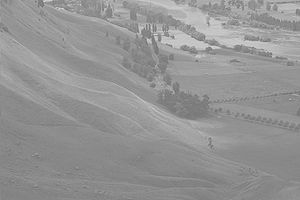
\includegraphics[width=0.3\textwidth]{Images/C original.jpg}
        \caption{Original image}
        \label{C original}
    \end{subfigure}
    \begin{subfigure}{\textwidth}
        \centering
        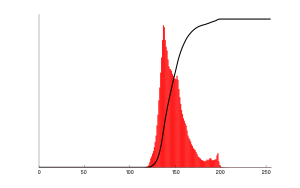
\includegraphics[width=0.3\textwidth]{Images/C original histogram.png}
        \caption{Histogram of original image}
        \label{C original histogram}
    \end{subfigure}
    \begin{subfigure}{\textwidth}
        \centering
        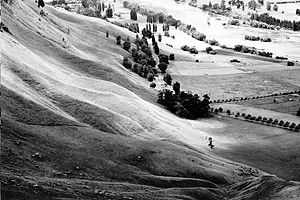
\includegraphics[width=0.3\textwidth]{Images/C equalised.jpg}
        \caption{Histogram-equalised image}
        \label{C equalised}
    \end{subfigure}
    \begin{subfigure}{\textwidth}
        \centering
        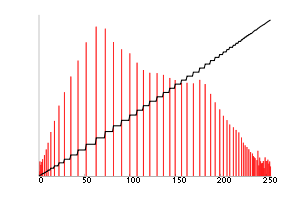
\includegraphics[width=0.3\textwidth]{Images/C equalised histogram.png}
        \caption{Histogram of histogram-equalised image}
        \label{C equalised histogram}
    \end{subfigure}
    \caption{Histogram and histogram equalisation \cite{Histogram equalisation wiki}}
    \label{Histogram and histogram equalisation}
\end{figure}

\subsection{Fast Fourier Transform}
The Fourier transform (FT) decomposes a function into its constituent frequencies, as illustrated in Figure \ref{FT}. The function in red is can be represented by a superposition of all the sinusoidal functions shown, each having a unique frequency and with magnitudes as indicated on the right panel. A function that changes more abruptly will have stronger high-frequency components than a smoother one. 

In image processing, the discrete Fourier transform (DFT) is often preferred, which takes a finite sequence of equally-spaced values as input and is thus better suited than the FT. It is defined by
\begin{equation}
    X_k = \sum_{n=0}^{N-1} x_n \cdot e^{-i2\pi kn/N}, \quad 0 \leq k \leq N-1
    \label{DFT}
\end{equation}
where $x_0,x_1,...,x_{N-1}$ is the input sequence and $X_0,X_1,...,X_{N-1}$ is the output sequence. $X_k$ is effectively the result of the dot product between the vector $[x_0,x_1,...,x_{N-1}]$ and $[e^0,e^{-i2\pi k/N},...,,e^{-i2\pi k(N-1)/N}]$, and the latter is a finite sequence of frequency $2\pi k$. Therefore, the DFT computes the magnitude of the component of the input sequence with frequency $2\pi k$, for $0 \leq k \leq N-1$.

Figure \ref{FFT on images} gives an example of FFT applied on a real image. The top row shows a set of images and the bottom row shows the corresponding transforms (amplitudes only). Points near the origin represent lower-frequency components and are cut off when a high-pass filter is applied to the image.

\begin{figure}
    \centering
    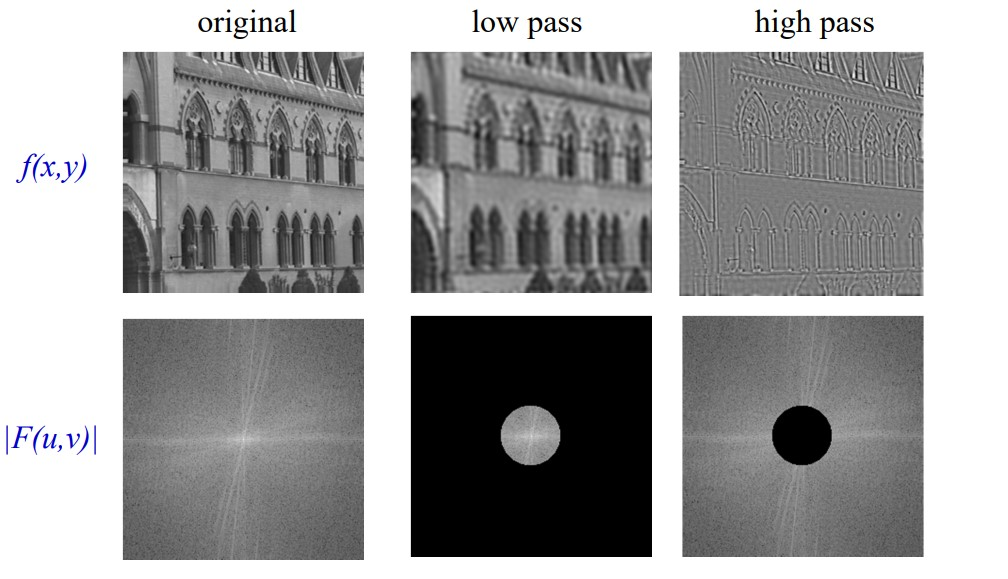
\includegraphics[width=0.3\textwidth]{Images/FFT on images.jpg}
    \caption{FFT and filtering on images \cite{Fourier transform lecture}}
    \label{FFT on images}
\end{figure}

A drawback of using Equation \ref{DFT} is that it has a time complexity of $O(N^2)$. In image processing, where the inputs are 2D sequences, the time complexity quickly explodes and makes the equation practically impossible to use. A fast Fourier transform (FFT) is an algorithm that computes the DFT with smaller timer complexity. There are many feasible algorithms and all known ones have complexity $O(N\log N)$ \cite{Fast Fourier transform wiki}. Detailed discussion on FFT algorithms is beyond the scope of this report.

\begin{figure}
    \centering
    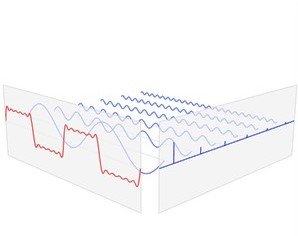
\includegraphics[width=0.3\textwidth]{Images/FT.jpg}
    \caption{Fourier transform \cite{Fourier transform wiki}}
    \label{FT}
\end{figure}

\subsection{Focusing and Astigmatism Correction}
The focusing and astigmatism of an SEM image can be evaluated using its FFT. Figure \ref{SEM astigmatism} provides a set of sample images that illustrate how different degrees of defocus and astigmatism affect the image and its FFT. An in-focus image contains more details, and its FFT will thus have stronger high-frequency components. As an astigmatic image goes from under-focus from over-focus, the elliptical incidence area of the electron probe rotates by 90 degrees and makes the image appear stretched in the new direction. As a result, its FFT also rotates by 90 degrees. K.H. Ong, J.C.H. Phang and J.T.L. Thong proposed an algorithm for automatic focusing and astigmatism correction \cite{SEM astigmatation correction algorithm} using these properties.

The FFT of an image can be converted into a binary image by applying a threshold to the magnitudes, and segmented into 8 regions as shown in Figure \ref{FFT regions}. A pixel has value 1 if the magnitude is above the threshold and 0 otherwise. Let $I$ be a matrix representing the current image with focal length set to $F$, obtain an under-focused image $I_{uf}$ and over-focused image $I_{of}$ by setting the focal length to $F-\Delta F=F_{uf}$ and $F+\Delta F=F_{of}$, respectively. Let $FI$, $FI_{uf}$ and $FI_{of}$ be matrices representing the binary FFT of $I$, $I_{uf}$ and $I_{of}$, respectively.

The focal length can be adjusted by comparing the sum of pixel values in $FI$, $FI_{uf}$ and $FI_{of}$. Let the perfect focal length for the image be $\hat{F}$, then
\begin{align*}
\begin{cases}
    \text{sum}(FI_{of}) < \text{sum}(FI) < \text{sum}(FI_{uf}), \quad & \hat{F} < F_{uf} \\
    \text{sum}(FI_{of}) < \text{sum}(FI),\ \text{sum}(FI_{of}) < \text{sum}(FI_{uf}), \quad & F_{uf} < \hat{F} < F \\
    \text{sum}(FI_{of}) = \text{sum}(FI_{uf}) < \text{sum}(FI), \quad & F=\hat{F} \\
    \text{sum}(FI_{uf}) < \text{sum}(FI),\ \text{sum}(FI_{uf}) < \text{sum}(FI_{of}), \quad & F_{of} > \hat{F} > F \\
    \text{sum}(FI_{uf}) < \text{sum}(FI) < \text{sum}(FI_{of}), \quad & \hat{F} > F_{of}
\end{cases}
\end{align*}
Let
\begin{equation}
    P = \text{sum}(FI_{of}) - \text{sum}(FI_{uf})
\end{equation}
Then, the rules for adjusting focal length are
\begin{itemize}
    \item when $P>0$, the focal length should be decreased.
    \item when $P<0$, the focal length should be increased.
\end{itemize}

After the focal length has been set to the perfect value, i.e. when $F=\hat{F}$, the stigmator settings can be determined by comparing the sum of pixel values in different regions of $FI$, $FI_{uf}$ and $FI_{of}$. The rules for adjustment can be determined using Figure \ref{SEM astigmatism}. Let
\begin{align}
    P_{R12} & = \text{sum}(FI_{of,R12}) - \text{sum}(FI_{uf,R12}) \\
    P_{R34} & = \text{sum}(FI_{of,R34}) - \text{sum}(FI_{uf,R34}) \\
    P_{S12} & = \text{sum}(FI_{of,S12}) - \text{sum}(FI_{uf,S12}) \\
    P_{S34} & = \text{sum}(FI_{of,S34}) - \text{sum}(FI_{uf,S34})
\end{align}
Then the rules for adjusting stigmator settings are
\begin{itemize}
    \item when $P_{R12}>0$ and $P_{R34}<0$, stigma x should be decreased.
    \item when $P_{R12}<0$ and $P_{R34}>0$, stigma x should be increased.
    \item when $P_{S12}>0$ and $P_{S34}<0$, stigma y should be increased.
    \item when $P_{S12}<0$ and $P_{S34}>0$, stigma y should be decreased.
\end{itemize}

Figure \ref{Correction algorithm flowchart} shows the general flow chart of the algorithm.

\begin{figure}
    \centering
    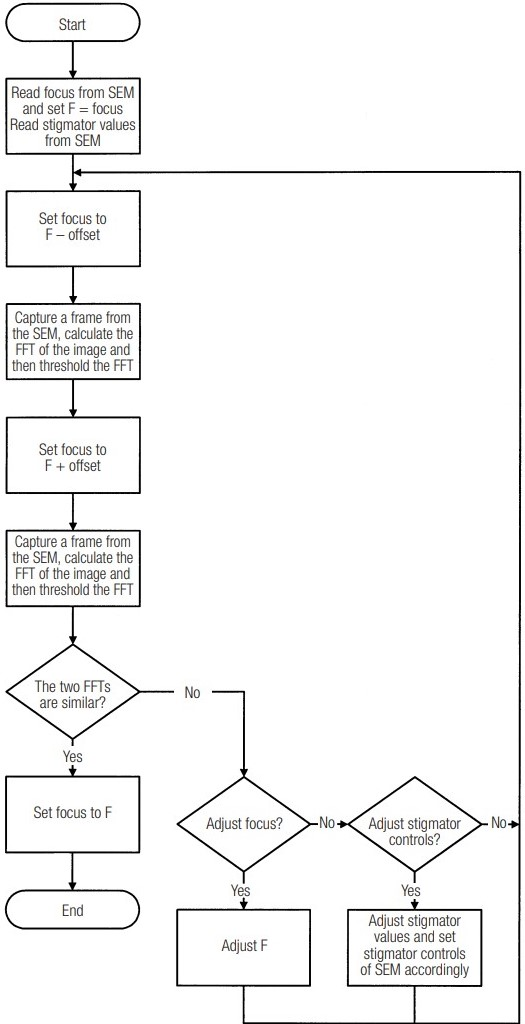
\includegraphics[width=0.7\textwidth]{Images/Correction algorithm flowchart.jpg}
    \caption{General flow chart of the correction algorithm \cite{SEM astigmatation correction algorithm}}
    \label{Correction algorithm flowchart}
\end{figure}

\begin{figure}
    \centering
    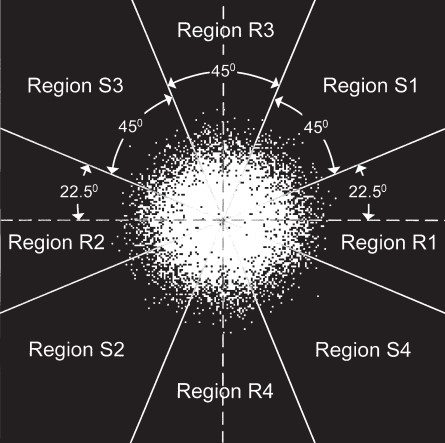
\includegraphics[width=0.9\textwidth]{Images/FFT regions.jpg}
    \caption{Segmented fast Fourier transform \cite{SEM astigmatation correction algorithm}}
    \label{FFT regions}
\end{figure}

\begin{figure}
    \centering
    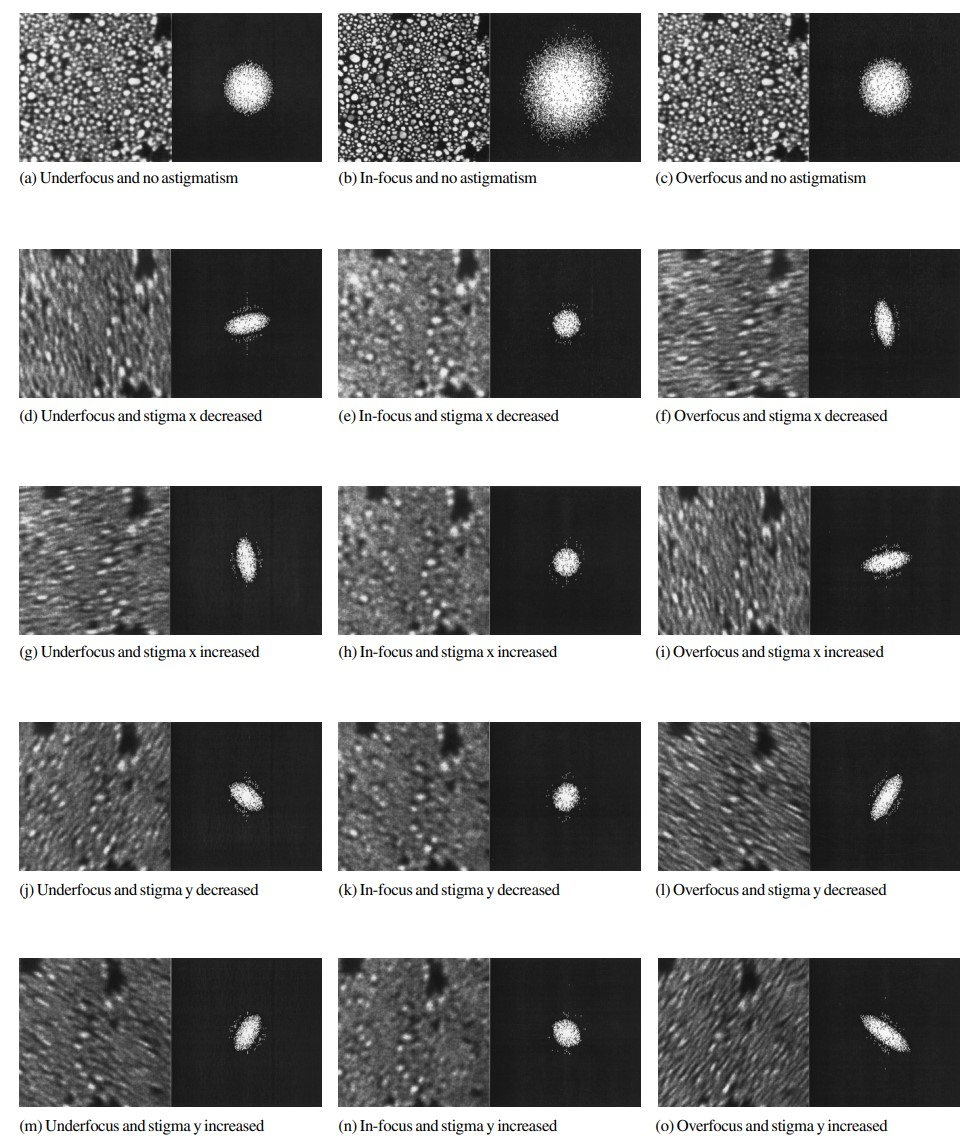
\includegraphics[width=0.9\textwidth]{Images/SEM astigmatism.jpg}
    \caption{Images of gold-on-carbon sample and their fast Fourier transforms (FFTs) for different degrees of defocus and astigmatism \cite{SEM astigmatation correction algorithm}}
    \label{SEM astigmatism}
\end{figure}

\section{The Software}
\subsection{Overview}
Overview of all modules.

\subsection{The SemImage Module}
Idea of the module.
Classes and functions.
Demo code.
Possible improvements.

\subsection{The SemTool Module}
Idea of the module.
Classes and functions.
Demo code.
Possible improvements.

\subsection{The SemCorrector Module}
Idea of the module.
Classes and functions.
Demo code.
Possible improvements.

\section{Demonstrations}
\subsection{Real-time Histogram Equalisation}
Screenshots of the software.
Demonstration of the algorithm.
Speed test of the algorithm.

\subsection{Real-time Fast Fourier Transform}
Screenshots of the software.
Demonstration of the algorithm.
Speed test of the algorithm.

\subsection{Automatic Focusing and Astigmatism Correction}
Screenshots of the software.
Demonstration of the algorithm.
Speed test of the algorithm.

\section{Next Steps}
Next steps.

\newpage
\begin{thebibliography}{}
    \bibitem{SEM A to Z}
    \textit{Scanning Electron Microscope A to Z}. JEOL Ltd. [Online]. Available: \url{https://www.jeol.co.jp/en/applications/pdf/sm/sem_atoz_all.pdf}. Accessed: May 9, 2020.

    \bibitem{SEM for semiconductor}
    T. Agemura and T. Sekiguchi, "Secondary electron spectroscopy for imaging semiconductor materials," 2018 International Symposium on Semiconductor Manufacturing (ISSM), Tokyo, Japan, 2018, pp. 1-3, doi: 10.1109/ISSM.2018.8651171.

    \bibitem{SEM astigmatation correction algorithm}
    K.H. Ong, J.C.H. Phang and J.T.L. Thong, "A robust focusing and astigmatism correction method for the scanning electron microscope," 1997, scanning 19: 553-563, doi: 10.1002/sca.4950190805.
    
    \bibitem{SEM wiki}
    "Scanning electron microscope." en.wikipedia.org. \url{https://en.wikipedia.org/wiki/Scanning_electron_microscope} (accessed May 9, 2020).

    \bibitem{Histogram equalisation wiki}
    "Histogram equalization." en.wikipedia.org. \url{https://en.wikipedia.org/wiki/Histogram_equalization} (accessed May 11, 2020).

    \bibitem{Fourier transform wiki}
    "Fourier transform." en.wikipedia.org. \url{https://en.wikipedia.org/wiki/Fourier_transform} (accessed May 12, 2020).

    \bibitem{Fast Fourier transform wiki}
    "Fast Fourier transform." en.wikipedia.org. \url{https://en.wikipedia.org/wiki/Fast_Fourier_transform} (accessed May 12, 2020).

    \bibitem{Fourier transform lecture}
    University of Oxford. (2014). 2D Fourier transforms and applications. [Online]. Available: \url{http://www.robots.ox.ac.uk/}

    \bibitem{SEM astigmatism correction}
    "Correcting Astigmatism in SEM Images." cambridge.org. \url{https://www.cambridge.org/core/journals/microscopy-today/article/correcting-astigmatism-in-sem-images/7ED43987C7916AAFBE1869522546AC84/core-reader} (accessed May 10, 2020).
\end{thebibliography}
\end{document}
